% articulo_6p.tex -- versión de 6 páginas con las correcciones de claridad y de citas
% (informe: ../informe_referencias_claridad.md). Compilar: pdflatex articulo_6p (x2).
% La figura 1 se toma de la página 3 del PDF de 6 páginas original (fig1_pagina.pdf).
\documentclass[10pt,letterpaper]{article}
\usepackage[utf8]{inputenc}
\usepackage[T1]{fontenc}
\usepackage{mathpazo}
\usepackage[scaled=0.92]{helvet}
\usepackage{microtype}
\usepackage{amsmath,amssymb,graphicx,booktabs,array}
\usepackage[left=1.7cm,right=1.5cm,top=1.6cm,bottom=1.9cm]{geometry}
\usepackage[super,sort&compress]{natbib}
\usepackage[font=small,labelfont={bf,sf},labelsep=period]{caption}
\usepackage[hidelinks]{hyperref}
\usepackage{titlesec,enumitem}
\titleformat{\section}{\normalfont\sffamily\bfseries\MakeUppercase}{\thesection.}{0.5em}{}
\titleformat{\subsection}{\normalfont\sffamily\bfseries}{\thesubsection.}{0.5em}{}
\titlespacing*{\section}{0pt}{9pt plus 2pt}{4pt}
\titlespacing*{\subsection}{0pt}{6pt plus 2pt}{3pt}
\renewcommand{\thesubsection}{\arabic{section}.\arabic{subsection}}
\setlength{\parskip}{0pt}
\setlength{\textfloatsep}{8pt plus 2pt minus 2pt}
\setlength{\floatsep}{6pt plus 2pt minus 2pt}
\setlength{\abovedisplayskip}{5pt plus 2pt minus 2pt}
\setlength{\belowdisplayskip}{5pt plus 2pt minus 2pt}
\renewcommand{\topfraction}{0.9}\renewcommand{\textfraction}{0.08}
\newcommand{\dc}{\delta_c}
\newcommand{\mr}{\langle r\rangle}
\newcommand{\ee}[2]{#1\times10^{#2}}
\newcommand{\dd}{\mathrm{d}}
\newcommand{\hb}{\hbar}
\renewcommand{\figurename}{Fig.}\renewcommand{\tablename}{Tabla}
\renewcommand{\refname}{\normalfont\sffamily\bfseries REFERENCIAS}

\begin{document}
\begin{flushleft}
{\sffamily\bfseries\LARGE Umbral de ligadura en un potencial tipo Yukawa: cruce de cajas y momento angular\par}
\vspace{6pt}
{\sffamily\bfseries Juan Sebastian Calixto Pernett$^{1}$, Luis Felipe Ramirez Andrade$^{2}$\par}
\vspace{2pt}
{\sffamily\footnotesize $^{1,2}$Departamento de Física, Facultad de Ciencias, Universidad Nacional de Colombia, Sede Bogotá\\
$^{1}$jcalixtop@unal.edu.co, $^{2}$luramirezan@unal.edu.co\par}
\vspace{4pt}
{\sffamily\footnotesize Compilado el 27 de noviembre de 2026\par}
\end{flushleft}
\vspace{-2pt}
\noindent\textsf{\textbf{Resumen:}} {\small Este artículo estudia el efecto del apantallamiento característico del potencial de Yukawa sobre la existencia del estado fundamental ligado. En unidades naturales ($\hb=m=g=1$) la dependencia queda toda en el parámetro adimensional $\delta=\mu\hb^2/(mg)$. El apantallamiento crítico $\dc$ para el cual deja de existir el estado 1s se conoce con muchas cifras~\cite{Rogers1970,Gebremedhin2023}; lo difícil es decidir, con un cálculo en caja finita, si un estado casi sin ligar existe o es un artefacto numérico. La energía $E_0(\delta)$ y el radio medio $\mr(\delta)$ se calculan con dos métodos independientes: un solucionador radial por diferencias finitas con extrapolación de Richardson y una integral de camino en tiempo imaginario, que trata la singularidad $-1/r$ con la acción de pares de Coulomb y el resto acotado, $W=(1-e^{-\delta r})/r$, con Trotter simétrico, de modo que el peso es real, positivo y normalizable. Se evalúa como matriz de transferencia (sin ruido estadístico). Ambos métodos se verifican con los casos exactos de Coulomb y Hulthén. Al tomar pares de cajas $(R,2R)$ se encuentra que las curvas de $y=2R^2E_0/\pi^2$ frente a $\delta$ se cruzan en un $\delta^*$ que converge a $\dc$ como $1/R^2$, con un coeficiente fijado por el rango efectivo, sin parámetros ajustables. Con la integral de camino resulta $1.19054410<\dc<1.19067723$, un intervalo 3 veces más estrecho que la ventana $1/(cR)$ que el signo de la energía deja sin clasificar con la misma caja mayor (55 veces si la extrapolación se aplica directamente al cruce). Con tres cajas pequeñas ($R\le200$), todas con energía positiva, el cruce clasifica correctamente $\delta=1.19$ como ligado. Se obtienen además los umbrales de los estados 2s, 2p y 3d ($\dc=0.310209$, $0.220217$ y $0.091345$); el radio medio de la onda~p crece como un logaritmo cuya pendiente es la amplitud de la cola a energía cero. El método se generaliza a $\ell\ge1$: la variable $y$ tiende a cero en el umbral (no tiene punto fijo no nulo), pero la variable $Y\propto R^{2\ell+1}E$ sí, y su cruce converge como $R^{-4\ell}$; el 2s sigue la ley $1/R^2$ del 1s. Con cruces de cajas, la integral de camino da $\dc(2p)=0.2202168059\pm\ee{8.6}{-9}$ y $\dc(2s)=0.31020963\pm\ee{8.4}{-6}$. Se reportan también los controles que no pasan.\par}

\section{Introducción}

Introducido en 1935 por Hideki Yukawa, el potencial que recibe su nombre, de la forma $V(r)=-g\,e^{-\mu r}/r$, describe una interacción de Coulomb apantallada~\cite{Yukawa1935}. Surgió de la necesidad de explicar las fuerzas entre nucleones: Yukawa combinó la noción de una interacción de corto alcance con el intercambio de partículas, lo cual se refleja en el decaimiento exponencial ($e^{-\mu r}$), con alcance $1/\mu$ fijado por la masa del mesón, y en la dependencia coulombiana ($1/r$). El mismo perfil aparece como apantallamiento de Debye y Hückel en plasmas.

Este potencial tiene un número finito de estados ligados, y cada uno desaparece al alcanzar un apantallamiento crítico. En unidades naturales el comportamiento depende totalmente del parámetro $\delta=\mu\hb^2/(mg)$, el cociente entre el tamaño atómico (radio de Bohr generalizado) y el alcance del potencial. Este artículo estudia el valor $\dc$ para el cual deja de existir el estado fundamental 1s y, sobre todo, cómo distinguir, cerca de ese valor, un estado débilmente ligado de un artefacto de la caja finita en la que se calcula. Finalmente se extiende el análisis al momento angular.

\textit{Lo ya conocido.} El valor de $\dc$ no es un resultado original de este trabajo. Rogers, Graboske y Harwood lo calcularon en 1970~\cite{Rogers1970}; después se refinó con métodos variacionales y numéricos~\cite{Gomes1994,Edwards2017} hasta $\dc=1.1906124207(2)$~\cite{Napsuciale2021PLB} y $1.19061242106\ldots$~\cite{Gebremedhin2023}. Aquí, la solución de energía cero, sin caja ni malla, da $\dc=1.1906124210606$, que coincide con este último en todas las cifras citadas; el valor de Edwards et al.~\cite{Edwards2017} queda $\ee{2.1}{-7}$ por debajo y se reporta como discrepante, sin afirmar la causa. También se conocen los exponentes con que la energía se anula, $(\dc-\delta)^2$ para $\ell=0$ y $(\dc-\delta)$ para $\ell\ge1$~\cite{KlausSimon1980,Serra1998}.

\textit{Contribuciones.} En la literatura consultada (revisión breve, no exhaustiva) no se encontró: (i)~el cruce de cajas de pared dura en onda~s aplicado al apantallamiento crítico, con coeficientes predichos por el rango efectivo y usado, con una integral de camino, como prueba de artefacto independiente del signo de la energía; (ii)~los coeficientes de $E$, $\mr$ y $\langle r^2\rangle$ en los umbrales 2s, 2p y 3d, y la variable de caja con punto fijo para $\ell\ge1$; (iii)~la ley de convergencia del cruce para $\ell\ge1$ y para el 2s. Los ingredientes existen por separado, y hay un antecedente cercano para $\ell=1$~\cite{SerraSpatial}; lo nuevo es su combinación, y no se puede afirmar que no exista en fuentes no consultadas.

\section{Marco teórico}
\subsection{Adimensionalización y cotas}

Con $a=\hb^2/(mg)$ como unidad de longitud y $mg^2/\hb^2$ como unidad de energía, la ecuación radial de la onda parcial $\ell$, con $u(r)=rR(r)$, es
\begin{equation}
-\tfrac12u''(r)+\Big[-\frac{e^{-\delta r}}{r}+\frac{\ell(\ell+1)}{2r^2}\Big]u(r)=E\,u(r),\qquad u(0)=0,\label{eq:radial}
\end{equation}
con $\kappa=\sqrt{-2E}$ y $\Delta=\dc-\delta$. Solo $\delta$ tiene significado físico: a $g$ y $m$ fijos, el umbral en $\mu$ es $\mu_c=\dc\,mg/\hb^2$. Para $\delta\to0$ se recupera el hidrógeno ($E_0=-1/2$, $\mr=3/2$). Cuatro cotas encierran el umbral del 1s: dos propias (una prueba $e^{-r/b}$ da ligado si $\delta<1$, y una de Ritz con 12 exponenciales da $\dc\ge1.19055$) y dos de la literatura: el criterio de Bargmann~\cite{Bargmann1952}, $n_0<2/\delta$, excluye el estado si $\delta\ge2$, y el de Schwinger~\cite{Schwinger1961} da $\dc\le2\sqrt{2\ln2-1}\approx1.24305$. Cerca del umbral $\kappa\simeq c\,\Delta$, es decir $E\simeq-(c\Delta)^2/2$ y $\mr\simeq1/(2\kappa)$, con $c=-\dd(1/a)/\dd\delta=0.741192$ calculada a energía cero.

\subsection{Integral de camino con acción de pares}

En tiempo imaginario $Z(\tau)\sim e^{-E_0\tau}$ y solo sobrevive el estado fundamental~\cite{FeynmanHibbs1965}. Se separa el potencial en la parte de Coulomb y un resto acotado,
\begin{equation}
V(r)=-\frac1r+W(r),\qquad W(r)=\frac{1-e^{-\delta r}}{r}\in[0,\delta].\label{eq:W}
\end{equation}
La discretización primitiva produce un factor $e^{+\epsilon/r}$ cuya integral sobre cualquier eslabón diverge en $r=0$ para todo $\epsilon>0$ y todo $\delta$: el peso es real y positivo, pero no normalizable, y el apantallamiento solo cambia una constante. Se usa entonces la acción de pares~\cite{PollockCeperley1984,Ceperley1995}, que incorpora el propagador exacto de Coulomb. El eslabón de la onda $\ell$ es
\begin{equation}
T_\ell(r,r';\epsilon)=K_\ell\,e^{-U_\ell}\,e^{-\epsilon[W(r)+W(r')]/2},\qquad
K_\ell=\frac{\sqrt{rr'}}{\epsilon}\,e^{-(r-r')^2/2\epsilon}\,\tilde I_{\ell+1/2}\Big(\frac{rr'}{\epsilon}\Big),\label{eq:T}
\end{equation}
con $\tilde I_\nu(z)=I_\nu(z)e^{-z}$, $K_\ell$ el núcleo libre exacto de la onda parcial y $U_\ell=-\ln(\rho_\ell/K_\ell)$, donde $\rho_\ell$ es el propagador exacto de Coulomb, tabulado numéricamente. La singularidad queda absorbida en $\rho_\ell$ y solo el resto $W$ se trata con factorización simétrica, con sesgo $O(\epsilon^2)$. El peso de un camino es real, positivo (ningún elemento de la matriz es negativo) y normalizable; no se suaviza el potencial. Con cuadratura de Nyström ($r_i=ih$) la energía es $E(\epsilon)=-\ln\lambda/\epsilon$, con $\lambda$ el mayor autovalor de la matriz en banda $h\,T_\ell(r_i,r_j)$ (autovector de signo constante, Perron y Frobenius) y el segundo para el 2s. La \emph{receta} de producción es: $h=0.04$ y $0.02$ con Richardson de exponente~4; $\epsilon=0.2$, $0.1$, $0.05$ con ley $\epsilon^2$; y una barra que suma linealmente la diferencia entre extrapolaciones y el sesgo de pared. Para un cruce de cajas hay dos variantes: \emph{A}, aplicar la receta a $E_0$ y propagarla al cruce (intervalo oficial), y \emph{B}, aplicarla directamente al cruce. $K_\ell$ es el núcleo del espacio libre: no incluye el término imagen que anularía el propagador en $r=R$. Por eso la pared solo actúa en los tiempos discretos y queda efectivamente en $R+\beta_w\sqrt\epsilon$, con $\beta_w=-\zeta(1/2)/\sqrt{2\pi}=0.5826$, valor que comprobamos numéricamente. La referencia independiente es el solucionador radial (diferencias finitas con Richardson y un disparo sin malla empalmado con la solución exterior exacta).

\begin{figure}[t]
\centering
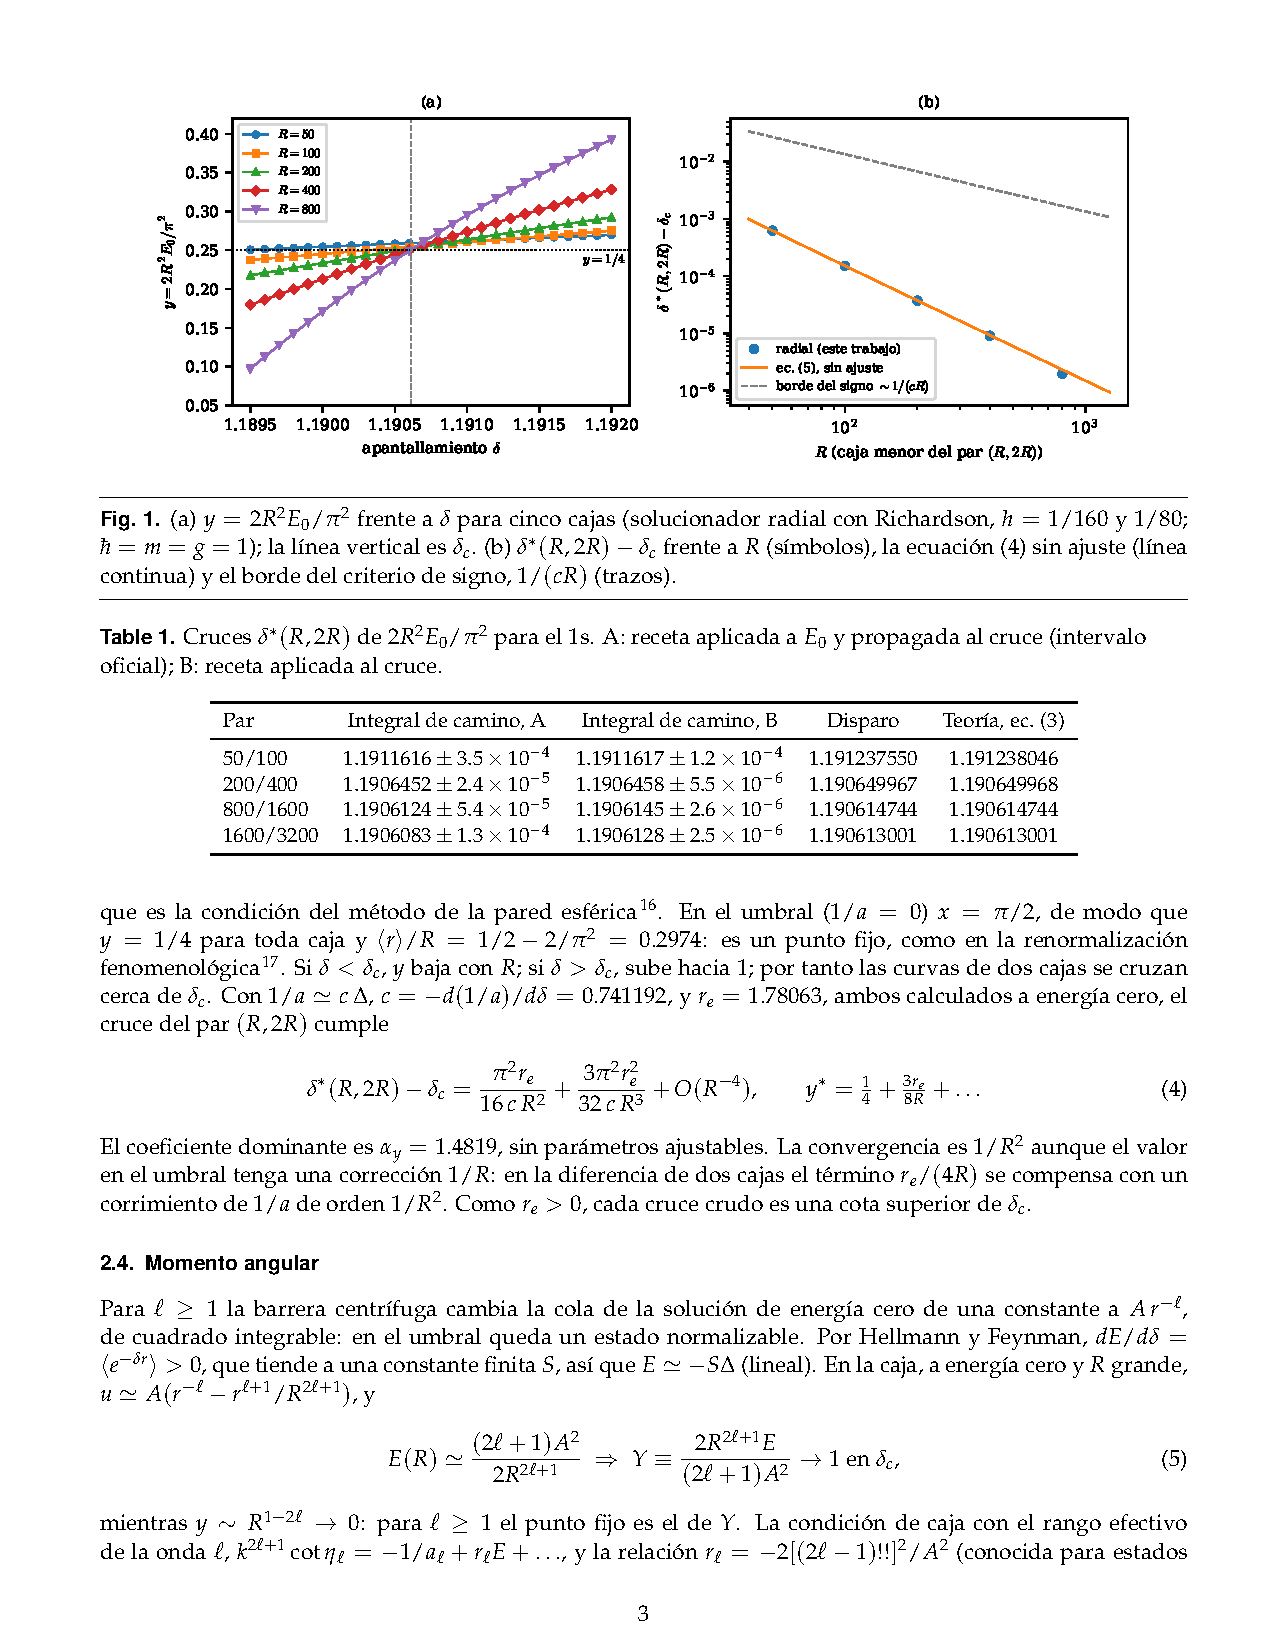
\includegraphics[width=0.93\textwidth,trim=62 566 74 36,clip]{fig1_pagina.pdf}
\caption{(a) $y=2R^2E_0/\pi^2$ frente a $\delta$ para cinco cajas (solucionador radial con Richardson, $h=1/160$ y $1/80$; $\hb=m=g=1$); la línea vertical es $\dc$. (b) $\delta^*(R,2R)-\dc$ frente a $R$ (símbolos), la ecuación~\eqref{eq:ley} sin ajuste (línea continua) y el borde del criterio de signo, $1/(cR)$ (trazos).}\label{fig:cruces}
\end{figure}

\begin{table}[t]
\centering\small
\caption{Cruces $\delta^*(R,2R)$ de $2R^2E_0/\pi^2$ para el 1s. A: receta aplicada a $E_0$ y propagada al cruce (intervalo oficial); B: receta aplicada al cruce.}\label{tab:cruces}
\begin{tabular}{lcccc}
\toprule
Par & Integral de camino, A & Integral de camino, B & Disparo & Teoría, ec.~\eqref{eq:caja}\\
\midrule
50/100    & $1.1911616\pm\ee{3.5}{-4}$ & $1.1911617\pm\ee{1.2}{-4}$ & 1.191237550 & 1.191238046\\
100/200   & $1.1907465\pm\ee{8.4}{-5}$ & $1.1907468\pm\ee{2.6}{-5}$ & 1.190764616 & 1.190764645\\
200/400   & $1.1906452\pm\ee{2.4}{-5}$ & $1.1906458\pm\ee{5.5}{-6}$ & 1.190649967 & 1.190649968\\
400/800   & $1.1906197\pm\ee{2.5}{-5}$ & $1.1906208\pm\ee{3.1}{-6}$ & 1.190621745 & 1.190621745\\
800/1600  & $1.1906124\pm\ee{5.4}{-5}$ & $1.1906145\pm\ee{2.6}{-6}$ & 1.190614744 & 1.190614744\\
1600/3200 & $1.1906083\pm\ee{1.3}{-4}$ & $1.1906128\pm\ee{2.5}{-6}$ & 1.190613001 & 1.190613001\\
\bottomrule
\end{tabular}
\end{table}

\subsection{Caja de Dirichlet y cruce de cajas}

En una esfera dura $u(R)=0$, y $\dd E/\dd R=-u'(R)^2/2<0$: la energía de la caja decrece con $R$ y nunca baja de la del espacio libre. Por eso el signo de $E$ solo se equivoca en un sentido (dice «no ligado» cuando sí hay estado) y lo hace hasta que $R$ supera la longitud de dispersión $a_s\propto1/\Delta$. Fuera del alcance del potencial $u=\sin(kr+\eta_0)$; la pared impone $\sin(kR+\eta_0)=0$ y, con $x=kR$ y el desarrollo de rango efectivo $k\cot\eta_0=-1/a+r_ek^2/2$~\cite{Bethe1949},
\begin{equation}
x\cot x=\frac Ra-\frac{r_e}{2R}\,x^2,\qquad y\equiv\frac{2R^2E_0}{\pi^2}=\frac{x^2}{\pi^2},\label{eq:caja}
\end{equation}
que es la condición del método de la pared esférica~\cite{Borasoy2007}. En el umbral ($1/a=0$) $x=\pi/2$, de modo que $y=1/4$ para toda caja y $\mr/R=1/2-2/\pi^2=0.2974$: es un punto fijo, como en la renormalización fenomenológica~\cite{Nightingale1976}. Si $\delta<\dc$, $y$ baja con $R$; si $\delta>\dc$, sube hacia~1; por tanto las curvas de dos cajas se cruzan cerca de $\dc$. Con $1/a\simeq c\Delta$ y $r_e=1.78063$, ambos calculados a energía cero, el cruce del par $(R,2R)$ cumple
\begin{equation}
\delta^*(R,2R)-\dc=\frac{\pi^2r_e}{16\,c\,R^2}+\frac{3\pi^2r_e^2}{32\,c\,R^3}+O(R^{-4}),\qquad y^*=\tfrac14+\frac{3r_e}{8R}+\dots\label{eq:ley}
\end{equation}
Los coeficientes son $\alpha_y=\pi^2r_e/(16c)=1.4819$ y $\beta_y=3\pi^2r_e^2/(32c)=3.958$, sin parámetros ajustables. En el umbral $y=\tfrac14+r_e/(4R)+\dots$, pero esa corrección $1/R$ no cambia la ley $1/R^2$ del cruce: en la diferencia de dos cajas se compensa con un corrimiento de $1/a$ de orden $1/R^2$. Como $r_e>0$, cada cruce crudo es una cota superior de $\dc$.

\subsection{Momento angular}

Para $\ell\ge1$ la barrera centrífuga cambia la cola de la solución de energía cero de una constante a $A\,r^{-\ell}$, de cuadrado integrable: en el umbral queda un estado normalizable. Por Hellmann y Feynman, $\dd E/\dd\delta=\langle e^{-\delta r}\rangle>0$, que tiende a una constante finita $S$, así que $E\simeq-S\Delta$ (lineal). En la caja, a energía cero y $R$ grande, $u\simeq A(r^{-\ell}-r^{\ell+1}/R^{2\ell+1})$, y
\begin{equation}
E(R)\simeq\frac{(2\ell+1)A^2}{2R^{2\ell+1}}\quad\Rightarrow\quad Y\equiv\frac{2R^{2\ell+1}E}{(2\ell+1)A^2}\to1\ \text{en}\ \dc,\label{eq:Y}
\end{equation}
mientras $y\sim R^{1-2\ell}\to0$: para $\ell\ge1$ el punto fijo es el de $Y$. La condición de caja con el rango efectivo de la onda $\ell$, $k^{2\ell+1}\cot\eta_\ell=-1/a_\ell+r_\ell E+\dots$, y la relación $r_\ell=-2[(2\ell-1)!!]^2/A^2$ (que derivamos y comprobamos numéricamente) dan, con $q=2^{1-2\ell}$ y $s=2^{2\ell+1}$ (factores que salen de comparar las cajas $R$ y $2R$),
\begin{equation}
\delta^*_y-\dc=\frac{(1-q)(2\ell+1)A^2}{6S}R^{-(2\ell+1)}[1+\dots],\qquad
\delta^*_Y-\dc=\frac{(1-q)\nu_\ell(2\ell+1)A^4}{2(s-1)S}R^{-4\ell}\Big[1-\frac{\gamma_Y}{R^2}+\dots\Big],\label{eq:cruce_l}
\end{equation}
con $\nu_\ell=(2\ell+1)^2/[(2\ell-1)(2\ell+3)]$ y $\gamma_Y$ el coeficiente de la primera corrección, que viene del término de forma del desarrollo de rango efectivo. El borde del criterio de signo es $\delta_0(R)-\dc=-(2\ell+1)A^2/(2SR^{2\ell+1})$; entonces, para $\ell\ge1$, el cruce de $y$ no mejora al signo y el de $Y$ gana $2\ell-1$ potencias de $R$. Para el 2s (segundo nivel de la caja en onda~s) rige la ley~\eqref{eq:ley} con las constantes del canal~s en $\dc(2s)$: $r_e=12.7714$, $c=1.31696$.

\section{Análisis y resultados}
\subsection{Punto de partida: la caja es el sistemático dominante}

El orden de Trotter medido va de 1.96 a 1.99 y el de la malla es 4.00; los casos exactos se reproducen (Coulomb a $\ee{2.2}{-7}$, Hulthén a $\ee{5}{-9}$~\cite{Varshni1990}) y los dos métodos coinciden en ocho valores de $\delta\in[0.2,1.19]$ con diferencia máxima $\ee{1.8}{-8}$. Sin extrapolar en $\epsilon$ el sesgo llega al 20\,\% de $|E_0|$ cerca del umbral, así que solo se usa la energía extrapolada. El caso difícil es $\delta=1.19$ ($a_s=+2204$): $E_0=+\ee{1.5}{-7}$ con $R=1600$ y $-\ee{7.1}{-8}$ con $R=3200$, así que el signo con $R\le1600$ diría «no ligado», y sería un error. Decide la localización: $\mr/R$ baja de $0.23$ ($R=3200$) a $0.043$ ($R=25600$), la fracción de densidad en $r<R/2$ sube de $0.90$ a $0.99999$ y $E_0$ se estabiliza en $-\ee{1.030}{-7}$ (la integral de camino da $-\ee{1.014}{-7}\pm\ee{2.3}{-8}$ en $R=12800$).

\subsection{Cruce de cajas en onda s}

La Fig.~\ref{fig:cruces}(a) muestra $y(\delta)$ para cinco cajas con el solucionador radial: todas las curvas pasan cerca de $1/4$ en el mismo $\delta$. La Fig.~\ref{fig:cruces}(b) y la Tabla~\ref{tab:cruces} comparan los cruces con la ecuación~\eqref{eq:ley}. La ecuación~\eqref{eq:caja}, resuelta sin desarrollar, coincide con el disparo a $\ee{2}{-9}$ o mejor desde el par 200/400, y los cocientes de diferencias sucesivas del disparo (4.125, 4.062, 4.031, 4.016) confirman la ley $1/R^2$. La integral de camino (método B) queda por debajo del disparo en los pares 50/100 a 400/800 en $-\ee{7.6}{-5}$, $-\ee{1.8}{-5}$, $-\ee{4.2}{-6}$ y $-\ee{9.4}{-7}$, frente a $-\ee{8.3}{-5}$, $-\ee{2.0}{-5}$, $-\ee{4.8}{-6}$ y $-\ee{1.18}{-6}$ que predice una pared efectiva en $R+c_w$, $c_w=0.1123$ (el residuo de extrapolar $\beta_w\sqrt\epsilon$ con la ley $\epsilon^2$).

Con 23 valores de $\delta$ en $[1.185,1.196]$ y $R=50,\dots,3200$, el ajuste ponderado $\delta^*=\dc+\alpha/R^2+\beta/R^3$ (pares con $R\ge100$) da, con la integral de camino,
\begin{equation}
1.19054410<\dc<1.19067723\ \ \text{(A)},\qquad 1.19060859<\dc<1.19061621\ \ \text{(B)}.\label{eq:intervalo}
\end{equation}
La comparación justa con el criterio de signo usa su resolución propia: una caja $R$ deja sin clasificar la ventana $0<\Delta<1/(cR)$, que mide $\ee{4.2}{-4}$ con $R=3200$. A igual caja mayor, el intervalo del cruce es 3.2 veces más estrecho (A) y 55 veces (B); si solo se usan cajas $R\le800$, 15 y 93 veces. El método A es más ancho porque la barra de $E_0$, al pasar a $y$, se multiplica por $R^2$.

\subsection{Prueba de artefacto en \texorpdfstring{$\delta=1.19$}{delta = 1.19}}

Hasta $R=1600$ los tres métodos dan $E_0>0$ (en $R=50$, $+\ee{5.0}{-4}$), que por el signo es «no ligado»; en cambio $y$ baja con $R$ desde el primer par. Esto solo no basta, pues el cruce crudo es una cota superior. Lo que clasifica es el cruce corregido con la ley~\eqref{eq:ley}, $\delta^*-\alpha_y/R^2-\beta_y/R^3$: con el par 50/100 vale 1.1906131 (disparo) y 1.1905372 (integral de camino), $\ee{6.1}{-4}$ y $\ee{5.4}{-4}$ por encima de 1.19; con la integral de camino ese margen es 1.5 veces la barra del método A y 4.7 la del B. Una variante no necesita constantes del umbral: con los cruces $\delta^*_1$ (50/100) y $\delta^*_2$ (100/200) y solo el exponente teórico~2, la extrapolación de Richardson da $\dc\simeq\delta^*_2-(\delta^*_1-\delta^*_2)/3=1.1906082\pm\ee{2.3}{-4}$ (A, 2.7 barras sobre 1.19) y $1.1906085\pm\ee{7.4}{-5}$ (B, 8.3 barras). Así se clasifica $\delta=1.19$ como ligado con cajas $R\le200$, todas de energía positiva.

\subsection{Umbrales y extensión espacial según \texorpdfstring{$\ell$}{l}}

Los umbrales salen de la raíz de $B(\delta)$ en la solución exterior a energía cero, $u=A\,r^{-\ell}+B\,r^{\ell+1}$: $\dc(2s)=0.3102092827139$, $\dc(2p)=0.2202168066066$ y $\dc(3d)=0.0913451207717$. Las leyes de la Tabla~\ref{tab:leyes} se calculan sin ajuste con pocos números del estado de umbral. Los exponentes medidos de $|E|$ frente a $\Delta$ son 2.0000003 (1s), 2.0000007 (2s), 1.00009 (2p) y 0.9999999 (3d). En la onda~p la norma es finita, pero la cola $A^2/r^2$ da a $\mr$ una contribución logarítmica: en el barrido, $\mr$ crece de 8.6 a 64.5 mientras $\kappa$ baja de 0.095 a $\ee{7.5}{-6}$, es lineal en $\ln(1/\kappa)$ con pendiente $6.597\pm0.001$ frente a $A^2=6.610$ predicha (la diferencia del 0.2\,\% es la corrección $O(\kappa\ln\kappa)$), y $\langle r^2\rangle\kappa\to5A^2/4=8.2627$ (medido 8.2629). En la onda~d, $\mr$ y $\langle r^2\rangle$ quedan finitos. Así, con $R=100$ el signo de $E$ es fiable desde $\Delta/\dc=\ee{1.1}{-2}$ en 1s pero ya desde $\ee{3.6}{-4}$ en 2p: la dificultad de caja es propia de $\ell=0$.

\begin{table}[t]
\centering\small
\caption{Leyes cerca del umbral ($\kappa=\sqrt{-2E}$, $\gamma$ constante de Euler) y constantes de energía cero. 1s: $c=0.741192$; 2p: $A^2=6.6102$, $S=0.126016$, $C_0=-13.428$; 3d: $A^2=16594$, $S=0.221917$, $\mr_0=21.616$.}\label{tab:leyes}
\begin{tabular}{cccc}
\toprule
$\ell$ & $E$ & $\mr$ & $\langle r^2\rangle$\\
\midrule
0 & $-(c\Delta)^2/2$ & $1/(2\kappa)$ & $1/(2\kappa^2)$\\
1 & $-S\Delta-(A^2/2)(2S\Delta)^{3/2}$ & $A^2\ln(1/\kappa)+C_0+A^2(\tfrac54-\gamma-\ln2)$ & $5A^2/(4\kappa)$\\
2 & $-S\Delta$ & $\mr_0-(A^2/3)\kappa^2\ln(1/\kappa)$ & $\langle r^2\rangle_0-\tfrac{35}{36}A^2\kappa$\\
\bottomrule
\end{tabular}
\end{table}

\begin{table}[t]
\centering\small
\caption{Leyes del cruce $\delta^*(R,2R)-\dc=\alpha R^{-p}$. Último exponente local medido (par 1600/3200 al 3200/6400) y $\alpha$ predicho sin ajuste.}\label{tab:leyes_cruce}
\begin{tabular}{cccccccc}
\toprule
Estado & Variable & Punto fijo & $p$ & $\alpha$ predicho & Exponente local & medido/pred.$-1$\\
\midrule
1s & $y$ & 1/4 & 2 & 1.48192 & 2.0012 & $+\ee{3}{-7}$\\
2s & $y$ & 1/4 & 2 & 5.98202 & 2.0087 & $+\ee{3.0}{-5}$\\
2p & $y$ & 0 & 3 & 13.1138 & 3.0063 & $+\ee{1.5}{-5}$\\
2p & $Y$ & 1 & 4 & 66.8706 & 4.0042 & $+\ee{2.9}{-3}$\\
3d & $y$ & 0 & 5 & 54523.4 & 5.0000 & $<10^{-7}$\\
3d & $Y$ & 1 & 8 & $\ee{1.04234}{8}$ & 7.9978 & $+\ee{1.3}{-6}$\\
\bottomrule
\end{tabular}
\end{table}

\subsection{Cruce de cajas generalizado}

Con el disparo sin malla ($R=25$ a 3200, hasta 6400 en precisión arbitraria) se hallaron 84 cruces, con el nivel aislado por conteo de nodos. La Tabla~\ref{tab:leyes_cruce} compara con las ecuaciones~\eqref{eq:cruce_l} y~\eqref{eq:ley}: los exponentes locales tienden a 2, 3, 4, 5 y 8, y los coeficientes, sin parámetro libre, aciertan entre $\ee{3}{-3}$ y menos de $10^{-7}$ en el par mayor. La ley $R^{-8}$ del 3d llega al piso numérico ($\approx\ee{4}{-16}$) en doble precisión (exponente local 7.85: ese control no pasa y así se reporta) y solo se confirma en precisión arbitraria (cocientes 249.7, 254.4 y 255.6 frente a 256).

Solo con cruces, sin usar la condición de energía cero, la integral de camino (receta sin cambios; 2s como segundo autovalor de la misma matriz, con un nodo y el mismo peso positivo) da
\begin{equation}
\dc(2p)=0.2202168059\pm\ee{8.6}{-9},\qquad\dc(2s)=0.31020963\pm\ee{8.4}{-6},\label{eq:dc_camino}
\end{equation}
frente a 0.22021680660657 y 0.31020928271394; ambas caen dentro de su barra. El 2s es tres órdenes menos preciso porque lo domina la pared. La prueba de artefacto se repite en la onda~p con cajas $R=25$, 50, 100: la energía es positiva en las tres para todo $\delta-\dc\in[-\ee{5}{-5},+\ee{2}{-4}]$, pero el signo de $D=Y(R)-Y(2R)$ distingue los dos lados. Con una barra que incluye el término siguiente de la ley~\eqref{eq:cruce_l}, el par 50/100 decide y acierta los 8 casos, mientras el par 25/50 solo decide 1 de 8 (ningún veredicto es erróneo). Sin las constantes del umbral, tres cajas (25, 50 y 100) y el exponente teórico~4 dan $\delta^*_2-(\delta^*_1-\delta^*_2)/15$ a $+\ee{6}{-9}\pm\ee{1.5}{-6}$ de $\dc(2p)$.

\subsection{Controles y limitaciones}

En total hay 471 controles: 395 pasan, 49 no pasan y 27 se midieron sin criterio previo o no aplican (lista en el repositorio). Los que no pasan se reportan así; cambiar el criterio después sería ajustarlo a los datos. Los principales sesgos de la integral de camino son la pared efectiva, $R_{\mathrm{ef}}=R+\beta_w\sqrt\epsilon-h/2$, y el corte de la banda de $T$ en $|r-r'|\le7\sqrt\epsilon$, que sube la energía en $+\ee{5}{-11}$. Limitaciones: la integral de camino solo cubre $\ell\le1$ y el 2s; las constantes $A^2$, $S$, $r_e$ y $c$ se calculan a energía cero, de modo que quien no conozca $\dc$ no las tiene (por eso las variantes sin constantes); y la discrepancia con Edwards et al.~\cite{Edwards2017} queda sin causa.

\section{Conclusiones}
\begin{enumerate}[leftmargin=*,itemsep=1pt,topsep=2pt]
\item La integral de camino con acción de pares, evaluada como matriz de transferencia, tiene peso real, positivo y normalizable para el Yukawa en $\ell=0$ y $\ell=1$ sin suavizar el potencial, y reproduce al solucionador radial; el sistemático dominante cerca del umbral es la caja.
\item En onda~s el cruce de dos cajas $(R,2R)$ de $2R^2E/\pi^2$ converge a $\dc$ como $\pi^2r_e/(16cR^2)$, sin parámetros libres. Con la integral de camino da $1.19054410<\dc<1.19067723$ y, con tres cajas $R\le200$ de energía positiva, clasifica $\delta=1.19$ como ligado, donde el signo necesitó $R=3200$ a $12800$.
\item El momento angular cambia el problema: para $\ell\ge1$ el estado de umbral es normalizable, $E$ es lineal en $\dc-\delta$, el radio medio de la onda~p crece como $A^2\ln(1/\kappa)$ y el de la onda~d queda finito; la dificultad de caja es propia de $\ell=0$.
\item El cruce se generaliza: para $\ell\ge1$ la variable con punto fijo es $Y\propto R^{2\ell+1}E$ y su cruce converge como $R^{-4\ell}$, frente a $R^{-(2\ell+1)}$ del signo y de $y$; el 2s sigue la ley del 1s.
\item Un estado débil se distingue de un artefacto de caja sin esperar a que la energía cambie de signo, declarando la resolución: en la onda~p, $10^{-5}$ en $\delta$ con dos cajas ($R=50$ y 100) y las constantes del umbral, o unos $\ee{1.5}{-6}$ con tres cajas y solo el exponente teórico.
\end{enumerate}

\noindent\textsf{\textbf{Uso de inteligencia artificial.}} El cálculo y la redacción se realizaron con un asistente de IA (Claude, de Anthropic) bajo la dirección del equipo, que fijó la pregunta, el plan y el enfoque. Hubo recálculo propio por bloque, revisión adversarial con otro agente, verificación bibliográfica y auditoría externa con otro modelo (Gemini). Las cifras salen de archivos escritos por el código, disponible en \url{https://github.com/luramirezan/integrales-camino-proyecto05}.

\begingroup\footnotesize\setlength{\itemsep}{0pt}
\begin{thebibliography}{18}\setlength{\itemsep}{0pt}\setlength{\parskip}{0pt}
\bibitem{Yukawa1935} Yukawa, H. (1935). On the interaction of elementary particles. I. \textit{Proc. Phys.-Math. Soc. Japan} 17, 48. Reimpreso en \textit{Prog. Theor. Phys. Suppl.} 1, 1 (1955). doi:10.1143/PTPS.1.1
\bibitem{Rogers1970} Rogers, F. J., Graboske, H. C. \& Harwood, D. J. (1970). Bound eigenstates of the static screened Coulomb potential. \textit{Phys. Rev. A} 1, 1577. doi:10.1103/PhysRevA.1.1577
\bibitem{Gomes1994} Gomes, O. A., Chacham, H. \& Mohallem, J. R. (1994). Variational calculations for the bound-unbound transition of the Yukawa potential. \textit{Phys. Rev. A} 50, 228. doi:10.1103/PhysRevA.50.228
\bibitem{Edwards2017} Edwards, J. P., Gerber, U., Schubert, C., Trejo, M. A. \& Weber, A. (2017). The Yukawa potential: ground state energy and critical screening. \textit{Prog. Theor. Exp. Phys.} 2017, 083A01. doi:10.1093/ptep/ptx107
\bibitem{Napsuciale2021PLB} Napsuciale, M. \& Rodríguez, S. (2021). Complete analytical solution to the quantum Yukawa potential. \textit{Phys. Lett. B} 816, 136218. doi:10.1016/j.physletb.2021.136218
\bibitem{Gebremedhin2023} Gebremedhin, D. \& Weatherford, C. (2023). First-order differential equations for single-particle quantum mechanical systems. \textit{Phys. Rev. E} 108, 045301. doi:10.1103/PhysRevE.108.045301
\bibitem{KlausSimon1980} Klaus, M. \& Simon, B. (1980). Coupling constant thresholds in nonrelativistic quantum mechanics. I. \textit{Ann. Phys.} 130, 251. doi:10.1016/0003-4916(80)90338-3
\bibitem{Serra1998} Serra, P., Neirotti, J. P. \& Kais, S. (1998). Finite-size scaling approach for the Schrödinger equation. \textit{Phys. Rev. A} 57, R1481. doi:10.1103/PhysRevA.57.R1481
\bibitem{SerraSpatial} Serra, P. A spatial finite size scaling method for calculation of critical parameters for weakly bound states. Manuscrito, \url{https://www.famaf.unc.edu.ar/~serra/serra28.pdf} (consultado el 23-11-2026; revista y año no comprobados).
\bibitem{Bargmann1952} Bargmann, V. (1952). On the number of bound states in a central field of force. \textit{Proc. Natl. Acad. Sci. USA} 38, 961. doi:10.1073/pnas.38.11.961
\bibitem{Schwinger1961} Schwinger, J. (1961). On the bound states of a given potential. \textit{Proc. Natl. Acad. Sci. USA} 47, 122. doi:10.1073/pnas.47.1.122
\bibitem{FeynmanHibbs1965} Feynman, R. P. \& Hibbs, A. R. (1965). \textit{Quantum Mechanics and Path Integrals}. McGraw-Hill, Nueva York.
\bibitem{PollockCeperley1984} Pollock, E. L. \& Ceperley, D. M. (1984). Simulation of quantum many-body systems by path-integral methods. \textit{Phys. Rev. B} 30, 2555. doi:10.1103/PhysRevB.30.2555
\bibitem{Ceperley1995} Ceperley, D. M. (1995). Path integrals in the theory of condensed helium. \textit{Rev. Mod. Phys.} 67, 279. doi:10.1103/RevModPhys.67.279
\bibitem{Bethe1949} Bethe, H. A. (1949). Theory of the effective range in nuclear scattering. \textit{Phys. Rev.} 76, 38. doi:10.1103/PhysRev.76.38
\bibitem{Borasoy2007} Borasoy, B., Epelbaum, E., Krebs, H., Lee, D. \& Meißner, U.-G. (2007). Two-particle scattering on the lattice: phase shifts, spin-orbit coupling, and mixing angles. \textit{Eur. Phys. J. A} 34, 185. doi:10.1140/epja/i2007-10500-9
\bibitem{Nightingale1976} Nightingale, M. P. (1976). Scaling theory and finite systems. \textit{Physica A} 83, 561. doi:10.1016/0378-4371(75)90021-7
\bibitem{Varshni1990} Varshni, Y. P. (1990). Eigenenergies and oscillator strengths for the Hulthén potential. \textit{Phys. Rev. A} 41, 4682. doi:10.1103/PhysRevA.41.4682
\end{thebibliography}
\endgroup
\end{document}
